\documentclass[conference]{IEEEtran}
% Template intent: IEEE conference-style paper scaffold for project communication.
\usepackage[T1]{fontenc}
\usepackage[utf8]{inputenc}
\usepackage{cite}
\usepackage{url}
\usepackage{graphicx}
\usepackage{booktabs}
\usepackage{amsmath}
\usepackage{tikz}
\usetikzlibrary{arrows.meta,positioning,shapes.geometric}

\title{Global Hazard Intel: A Multi-Source Environmental Hazard Intelligence System for Atmospheric, Health, and Earth-Observation Analytics}

\author{
\IEEEauthorblockN{Brian Gill}
\IEEEauthorblockA{
BG Code Tech\\
Email: briang.gill@bgcode.tech
}
}

\begin{document}
\maketitle

\begin{abstract}
Global Hazard Intel is a live environmental hazard intelligence platform that integrates weather observations, air-quality diagnostics, geocoded location queries, satellite-imagery context, and NASA event streams into a unified hazard monitoring workflow. The system is designed to support weather-station operators, public-health analysts, and earth-observation researchers through a shared operational interface with sector-specific analytics. This paper presents the system architecture, live data fusion strategy, analytics layers, desktop situational-awareness workflow, and report-generation design for decision support across dust storms, wildfire smoke, chemical emissions anomalies, and pollution spikes.
\end{abstract}

\begin{IEEEkeywords}
environmental intelligence, hazard detection, air quality, remote sensing, NASA, public health, weather analytics
\end{IEEEkeywords}

\section{Introduction}
Environmental hazard monitoring is increasingly dependent on the fusion of atmospheric measurements, remote-sensing signals, and public-health indicators. Operational users often work in fragmented tooling: meteorological teams prioritize wind and cloud transport, health agencies focus on exposure metrics, and earth-observation analysts track event signatures and geospatial context. Global Hazard Intel addresses this fragmentation with a single live monitoring environment that provides shared situational awareness while preserving sector-specific analytics.

\section{System Objective}
The platform targets four environmental hazard classes:
\begin{itemize}
    \item dust transport and dust storm activity
    \item wildfire smoke and transboundary plume movement
    \item chemical or industrial emissions anomalies
    \item acute pollution spikes in urban and regional settings
\end{itemize}

\section{Architecture}
Figure~\ref{fig:architecture} summarizes the end-to-end system design.

\begin{figure}[!t]
\centering
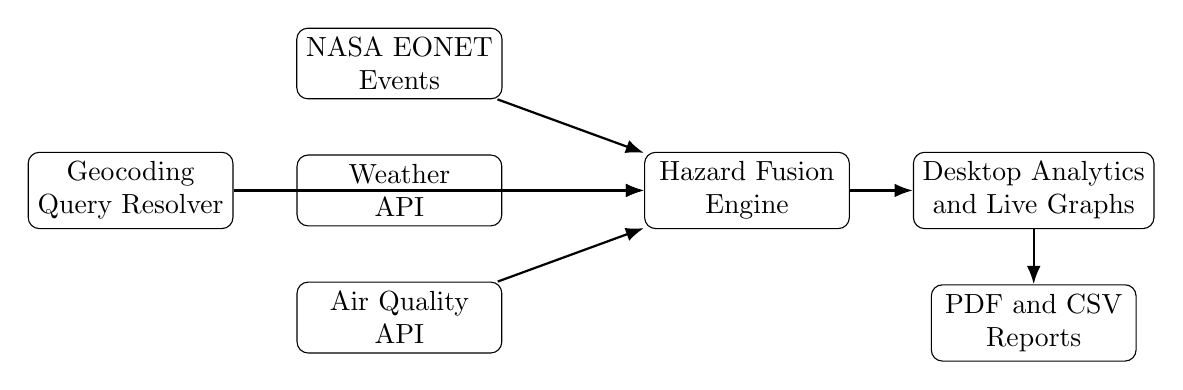
\begin{tikzpicture}[
    node distance=7mm and 8mm,
    block/.style={draw, rounded corners, minimum width=2.6cm, minimum height=0.85cm, align=center},
    line/.style={-Latex, thick}
]
\node[block] (geo) {Geocoding \\ Query Resolver};
\node[block, right=of geo] (weather) {Weather \\ API};
\node[block, below=of weather] (air) {Air Quality \\ API};
\node[block, above=of weather] (nasa) {NASA EONET \\ Events};
\node[block, right=18mm of weather] (fusion) {Hazard Fusion \\ Engine};
\node[block, right=of fusion] (desktop) {Desktop Analytics \\ and Live Graphs};
\node[block, below=of desktop] (reports) {PDF and CSV \\ Reports};

\draw[line] (geo) -- (fusion);
\draw[line] (weather) -- (fusion);
\draw[line] (air) -- (fusion);
\draw[line] (nasa) -- (fusion);
\draw[line] (fusion) -- (desktop);
\draw[line] (desktop) -- (reports);
\end{tikzpicture}
\caption{Global Hazard Intel dataflow and analytics architecture.}
\label{fig:architecture}
\end{figure}

\section{Data Sources}
The current implementation uses public live data services for rapid operational prototyping:
\begin{itemize}
    \item Open-Meteo geocoding and weather endpoints for location resolution and current meteorology~\cite{openmeteo_weather}
    \item Open-Meteo air-quality endpoints for AQI, particulates, and pollutant concentrations~\cite{openmeteo_air}
    \item NASA EONET for active event context in the search bounding box~\cite{nasa_eonet}
    \item OpenStreetMap Nominatim for exact address resolution~\cite{nominatim}
\end{itemize}

\section{Hazard Fusion Strategy}
Hazard inference is produced through weighted heuristics over live signals. Dust activity is driven by dust loading and wind transport; wildfire smoke risk combines event activity and particulate loading; chemical anomaly risk fuses sulfur dioxide, carbon monoxide, and nitrogen dioxide; pollution spikes weight AQI and particulate concentrations. These hazard-specific scores are mapped to severity and confidence outputs for operational consumption.

\section{Sector-Specific Analytics}
\subsection{Weather Analytics}
The weather analytics pane is designed for meteorological and weather-station workflows. It tracks near-surface wind speed, gust magnitude, directional transport, cloud cover, precipitation, and an operational weather score that reflects transport and instability conditions.

\subsection{Public Health Analytics}
The health analytics pane prioritizes exposure-relevant indicators such as US AQI, European AQI, PM$_{2.5}$, PM$_{10}$, ozone, and nitrogen dioxide. A public-health exposure score is derived to support respiratory-risk review and advisory escalation.

\subsection{Scientific Analytics}
The scientific pane summarizes the observation bounding box, counts NASA events within the query footprint, and computes an observation utility score intended for remote-sensing and atmospheric-science interpretation.

\section{Desktop Monitoring Workflow}
The desktop application opens with structured query modes for continent, country, city, address, or direct coordinates. Once the operator starts live detection, the system polls public data feeds on a configurable interval and updates:
\begin{itemize}
    \item hazard severity charts
    \item temporal trend lines
    \item satellite-imagery map context
    \item weather, health, and scientific analytics tabs
\end{itemize}
Each reporting action exports a new timestamped folder containing PDF and CSV artifacts for auditability and downstream review.

\section{Operational Relevance}
Global Hazard Intel is intentionally positioned for multi-stakeholder adoption:
\begin{itemize}
    \item \textbf{World health and air-quality agencies:} exposure monitoring, AQI escalation, and respiratory-risk triage
    \item \textbf{Weather stations and forecast offices:} transport diagnostics, plume motion review, and operational weather interpretation
    \item \textbf{NASA and scientific institutions:} event-context review, earth-observation alignment, and geospatial situational awareness
\end{itemize}

\section{Future Work}
Future iterations should replace heuristic scoring with validated spatiotemporal models, add geospatial databases for event persistence, integrate authenticated satellite products, and support ensemble forecasting for hazard spread and exposure estimation.

\section{Conclusion}
Global Hazard Intel demonstrates a practical path toward a unified hazard intelligence environment that serves operational meteorology, public-health analysis, and remote-sensing science in one system. Its architecture emphasizes live data fusion, transparent sector analytics, and exportable reporting, making it a strong base for further institutional and enterprise development.

\bibliographystyle{IEEEtran}
\bibliography{references}

\end{document}
